
\documentclass[a4paper]{article}
\usepackage{amsmath}

\usepackage{tikz}
\usetikzlibrary{bayesnet}


\begin{document}
\pagestyle{empty}

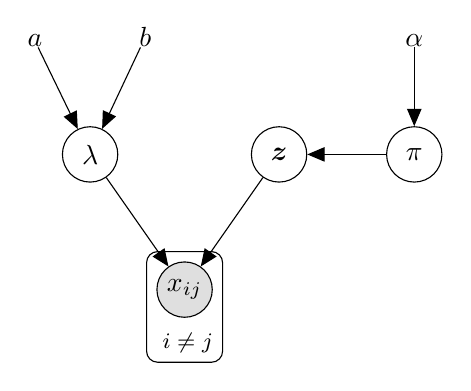
\begin{tikzpicture}
    \node[obs]                      (x_ij) {$x_{ij}$};
    \node[latent, above=of x_ij, xshift=1.2cm]    (z)    {$\boldsymbol{z}$};
    \node[latent, above=of x_ij, xshift=-1.2cm]   (lambda) {$\lambda$};
    \node[latent, right=of z] (pi) {$\pi$};
    \node[const,above=of pi] (alpha) {$\alpha$};
    \node[const, above=of lambda, xshift=-0.7cm] (a) {$a$};
    \node[const, above=of lambda, xshift=0.7cm] (b) {$b$};

    \edge{pi}{z};
    \edge{lambda, z}{x_ij};
    \edge{alpha}{pi};
    \edge{a,b}{lambda};

    \plate{}{(x_ij)}{$i\neq j$};
\end{tikzpicture}
\end{document}